\documentclass[11pt,xcolor={dvipsnames},hyperref={pdftex,pdfpagemode=UseNone,hidelinks,pdfdisplaydoctitle=true},usepdftitle=false]{beamer}
\usepackage{presentation}

\usepackage{tikz}
\usepackage{tikz-cd}

\usetikzlibrary{arrows,
	arrows.meta,
  backgrounds,
	bending,
	calc,
	decorations,
  decorations.markings,
	decorations.pathmorphing,
  fit,
  hobby,
	matrix,
	shapes}

\newcommand{\Exit}{\text{Exit}}

\newcommand{\circlestratone}{%
  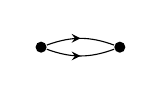
\begin{tikzpicture}[baseline=0,decoration={markings, mark=at position 0.5 with {\arrow{stealth}}}]
    \tikzstyle{vertex}=[circle,fill=black,minimum size=4pt,inner sep=0pt]
    \node[vertex] (v_1) at (-0.5,0) {};
    \node[vertex] (v_2) at (0.5,0) {};
    \draw[postaction=decorate] (v_1) to[out=20,in=160] (v_2);
    \draw[postaction=decorate] (v_1) to[out=-20,in=-160] (v_2);
    \node[fit=(current bounding box),inner sep=1mm]{};
  \end{tikzpicture}%
}

\newcommand{\circlestrattwo}{%
  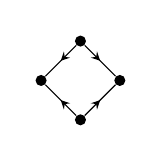
\begin{tikzpicture}[baseline=0,decoration={markings, mark=at position 0.5 with {\arrow{stealth}}}]
    \tikzstyle{vertex}=[circle,fill=black,minimum size=4pt,inner sep=0pt]
    \node[vertex] (v_3) at (-0.5,0) {};
    \node[vertex] (v_4) at (0.5,0) {};
    \node[vertex] (v_1) at (0,-0.5) {};
    \node[vertex] (v_2) at (0,0.5) {};
    \draw[postaction=decorate] (v_1) -- (v_3);
    \draw[postaction=decorate] (v_2) -- (v_3);
    \draw[postaction=decorate] (v_1) -- (v_4);
    \draw[postaction=decorate] (v_2) -- (v_4);
    \node[fit=(current bounding box),inner sep=1mm]{};
  \end{tikzpicture}%
}

\newcommand{\pointedplane}{%
  \begin{tikzpicture}[decoration={markings, mark=at position 0.5 with {\arrow{stealth}}}]
    \tikzstyle{vertex}=[circle,fill=black,minimum size=4pt,inner sep=0pt]
    \node[vertex] (v_1) at (0,0) {};
    \node[vertex] (v_2) at (1,0) {};
    \draw[postaction=decorate] (v_2) to[in=45,out=-45,loop] (v_2); 
    \draw[postaction=decorate] (v_1) -- (v_2);
    \node[fit=(current bounding box),inner sep=1mm]{};
  \end{tikzpicture}
}

\newcommand{\spherestratone}{%
  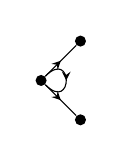
\begin{tikzpicture}[decoration={markings, mark=at position 0.5 with {\arrow{stealth}}}]
    \tikzstyle{vertex}=[circle,fill=black,minimum size=4pt,inner sep=0pt]
    \node[vertex] (v_1) at (0,0) {};
    \node[vertex] (v_2) at (0.5,-0.5) {};
    \node[vertex] (v_3) at (0.5,0.5) {};
    \draw[,postaction=decorate] (v_1) to[in=-45,out=45,loop] (v_1); 
    \draw[postaction=decorate] (v_1) -- (v_2);
    \draw[postaction=decorate] (v_1) -- (v_3);
    \node[fit=(current bounding box),inner sep=1mm]{};
  \end{tikzpicture}
}

\newcommand{\spherestrattwo}{%
  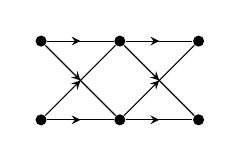
\begin{tikzpicture}[decoration={markings, mark=at position 0.5 with {\arrow{stealth}}}]
    \tikzstyle{vertex}=[circle,fill=black,minimum size=4pt,inner sep=0pt]
    \node[vertex] (v_1) at (0,-0.5) {};
    \node[vertex] (v_2) at (0,0.5) {};
    \node[vertex] (v_3) at (1,-0.5) {};
    \node[vertex] (v_4) at (1,0.5) {};
    \node[vertex] (v_5) at (2,-0.5) {};
    \node[vertex] (v_6) at (2,0.5) {};
    \draw[postaction=decorate] (v_1) -- (v_3);
    \draw[postaction=decorate] (v_1) -- (v_4);
    \draw[postaction=decorate] (v_2) -- (v_3);
    \draw[postaction=decorate] (v_2) -- (v_4);
    \draw[postaction=decorate] (v_3) -- (v_5);
    \draw[postaction=decorate] (v_3) -- (v_6);
    \draw[postaction=decorate] (v_4) -- (v_5);
    \draw[postaction=decorate] (v_4) -- (v_6);
    \node[fit=(current bounding box),inner sep=1mm]{};
  \end{tikzpicture}
}


% Enter presentation title to populate PDF metadata:
\hypersetup{pdftitle={The geometry of infinity-categories}}

% Enter path to PDF file with figures:
\newcommand{\pdf}{figures.pdf}

\begin{document}

% Enter title:
\title{The geometry of $\infty$-categories}

\information
%
% Enter URL to research paper (can be commented out):
%
% Enter authors:
{Clark Barwick}
%
% Enter location and date (can be commented out):
{London Mathematical Society -- 4 July 2025}

\frame{\titlepage}

\begin{frame}
  \frametitle{A crease}
  Take a piece of paper; fold it down the middle, creating a sharp crease.
  \includegraphics[scale=0.2,page=1]{\pdf}
  
  The \textsb{topology} of the paper has not changed, but the \textsb{geometry} has:

  at points on the crease, things like derivatives no longer work!

  You have introduced a \textsb{singular locus}.
\end{frame}

\begin{frame}
  \frametitle{Two creases}
  Fold your piece of paper again, perpindicular to the original fold.
  \includegraphics[scale=0.2,page=2]{\pdf}

  Still the topology hasn't changed.

  You've changed the geometry by introducing a new singular locus, and

  in the process, you've also made that point in the center \textsb{more singular}.
\end{frame}

\begin{frame}
  \frametitle{Stratifications: the idea}
  A \textsb{stratification} of a topological space $X$ partitions it
  into locally closed subsets $X_i \subseteq X$ -- called \emph{strata}.

  These arose in work of Whitney, Thom, and Mather in order to cope with complicated singular loci in higher dimensions. 
\end{frame}

\begin{frame}
  \frametitle{Stratifications: pictures}  
  \includegraphics<1>[scale=0.4,page=4]{\pdf}%
  \includegraphics<2>[scale=0.4,page=5]{\pdf}%
\end{frame}

\begin{frame}
  \frametitle{Stratifications: the general topology approach}
  Let $P$ be a \textsb{poset}.
  We declare $U \subseteq P$ \textsb{open} iff,
  \[
    (a \in U\ \&\ a \leq b) \implies b \in U
  \]

  \begin{example}
    In $[1] \coloneq \{0 < 1\}$, the point $0$ is closed, but $1$ is not.
  \end{example}

  Now a \textsb{stratified topological space} $X/P$ consists of:
  \begin{itemize}
    \item a topological space $X$,
    \item a poset $P$, and
    \item a continuous map $f \colon X \to P$.
  \end{itemize}
  The fiber $X_a = f^{-1}\{a\}$ is called the \textsb{$a$-th stratum}.
\end{frame}

\begin{frame}
  \frametitle{Stratifications: two strata}
  \begin{example}
    A stratification of $X$ over the poset $[1] = \{0 < 1\}$ is a decomposition $X = X_0 \cup X_1$, in which:
    \begin{itemize}
      \item the $0$-th stratum $X_0$ is closed, and
      \item the $1$-st stratum $X_1$ is the open complement.
    \end{itemize}
    \includegraphics[scale=0.2,page=6]{\pdf}%
  \end{example}
\end{frame}

\begin{frame}
  \frametitle{Stratifications: incomparable strata}
  \begin{example}
    If $P$ is a trivial poset (i.e., every pair of elements is incomparable), then
    a stratification of $X$ over $P$ is a decomposition of $X$ as a disjoint union of clopens $X_a$ for $a \in P$.

    \includegraphics[scale=0.25,page=7]{\pdf}%
  \end{example}
\end{frame}

\begin{frame}
  \frametitle{Stratifications: less trivial example}
  \begin{example}
    We can stratify the \textsb{corner} $[0,1)^n$ via the map
    $[0,1)^n \to [n] \coloneq \{0 < \dots < n\}$
    that carries $t$ to the largest $i$ such that $t_i \neq 0$.

    \includegraphics[scale=0.3,page=8]{\pdf}%
  \end{example}
\end{frame}

\begin{frame}
  \frametitle{Stratifications: circle}
  \begin{example}
    Stratify $S^0$ over the trivial poset $\{-1, +1\}$.

    Now let's \textsb{suspend} this to stratify $S^1$:

    \includegraphics[scale=0.2,page=9]{\pdf}
    \[
       \circlestrattwo
    \]
  \end{example}
\end{frame}
   
\begin{frame}
  \frametitle{Stratifications: sphere}
  \begin{example}
    Let's suspend again.
    Now we have a stratification of $S^2$:

    \includegraphics[scale=0.2,page=10]{\pdf}%
    \[
      \spherestrattwo
    \]
  \end{example}
\end{frame}

\begin{frame}
  \frametitle{Exit paths}
  There's an \textsb{$\infty$-category} attached to $X/P$:
  \begin{itemize}
    \item an object is a point of $X$
    \item a morphism from one point to another is an \textsb{exit path}:
      \includegraphics[scale=0.2,page=11]{\pdf}%
    \item a $2$-morphism is a \textsb{homotopy} of exit paths
    \item etc.
  \end{itemize}
  This is the \textsb{exit-path $\infty$-category} $\Exit(X/P)$.
\end{frame}

\begin{frame}
  \frametitle{Exit paths: examples}
  \begin{tabular*}{\textwidth}{@{\extracolsep\fill}lcccc}
  \toprule
    Poset & Stratification & Exit-path $\infty$-category\\
  \midrule
    $[n]$ & \raisebox{-0.5\totalheight}{\includegraphics[scale=0.15,page=8]{\pdf}} & $[n]$ \\ 
    $[1]$ & \raisebox{-0.5\totalheight}{\includegraphics[scale=0.15,page=12]{\pdf}} & $\circlestratone$\\ 
  \bottomrule
  \end{tabular*}
\end{frame}

\begin{frame}
  \frametitle{Exit paths: examples}
  \begin{tabular*}{\textwidth}{@{\extracolsep\fill}lcccc}
  \toprule
    Poset & Stratification & Exit-path $\infty$-category\\
  \midrule
    $\circlestrattwo$ & \raisebox{-0.5\totalheight}{\includegraphics[scale=0.15,page=9]{\pdf}} & $\circlestrattwo$\\ 
    $[1]$ & \raisebox{-0.5\totalheight}{\includegraphics[scale=0.15,page=13]{\pdf}} & $\pointedplane$ \\
  \bottomrule
  \end{tabular*}
\end{frame}

\begin{frame}
  \frametitle{Exit paths: examples}
  \begin{tabular*}{\textwidth}{@{\extracolsep\fill}lcccc}
  \toprule
    Poset & Stratification & Exit-path $\infty$-category\\
  \midrule
    $[1]$ & \raisebox{-0.5\totalheight}{\includegraphics[scale=0.15,page=6]{\pdf}} & $\spherestratone$ \\
    $\spherestrattwo$ & \raisebox{-0.5\totalheight}{\includegraphics[scale=0.15,page=10]{\pdf}} & $\spherestrattwo$ \\
  \bottomrule
  \end{tabular*}
\end{frame}

\begin{frame}
  \frametitle{These aren't all $1$-categories}
    \includegraphics[scale=0.2,page=14]{\pdf}

    There are two strata, each of which is contractible.
    That means there are two objects, neither of which has automorphisms.
    But the space of ways to exit from the yellow point into the green region is an $S^1$.

    In other words, $\Exit(S^2/[1])$ is a $2$-category with
    \begin{itemize}
      \item two objects $x_0$ and $x_1$
      \item only one interesting morphism, which goes $\gamma \colon x_0 \to x_1$
      \item countably many $2$-isomorphisms from $\gamma$ to itself.
    \end{itemize}
\end{frame}

\begin{frame}
  \frametitle{This works for a sphere in any dimension}
  This story works for any sphere actually:

  stratify $S^n$ over $[1]$ so that
  \begin{itemize}
    \item the $0$-th stratum is a single point
    \item the $1$-st stratum is everything else.
  \end{itemize}
  Now $\Exit(S^n/[1])$ has two objects $x_0$ and $x_1$,
  with $\text{Map}(x_0, x_1) = S^{n-1}$ and no other nontrivial maps.

  In particular, for $n \geq 3$,
  \textsb{these are not $n$-categories for any finite $n$}!
\end{frame}

\begin{frame}
  \frametitle{The homotopy theorem}
  \begin{theorem}[Ayala--Francis--Rozenblyum (2019), Haine (2018)]
    Let $E$ be an $\infty$-category in which every endomorphism is an automorphism.

    Then there is a stratified topological space $X/P$, unique up to stratified homotopy equivalence,
    such that
    \[
      E = \Exit(X/P) 
    \]

    Furthermore, this construction can be performed functorially.
  \end{theorem}
  In other words, \textsb{these $\infty$-categories are stratified homotopy types}.
\end{frame}

\begin{frame}
  \frametitle{Exodromy}
  \begin{theorem}[Lurie (2012), Haine--Porta--Teyssier (2024)]
    Let $X/P$ be a \textsb{reasonable} stratified topological space, and

    let $C$ be a \textsb{reasonable} category of coefficients.

    Then there is an equivalence of categories
    \[
      \text{Constr}(X/P, C) \simeq \text{Fun}(\Exit(X/P),C)
    \]
  \end{theorem}
  \includegraphics[scale=0.1,page=11]{\pdf}%
\end{frame}

\begin{frame}
  \frametitle{Beyond}
  Stratified homotopy types also make sense in \textsb{algebraic geometry}, particularly for the \textsb{étale topology}.

  $\text{Spec}\ \mathbf{Z}$ looks something like this as a stratified space:
  \includegraphics[scale=0.1,page=13]{\pdf}%
\end{frame}

\begin{frame}
\frametitle{Collection of figures (one figure per click)}
\includegraphics<1>[scale=0.275,page=1]{\pdf}%
\includegraphics<2>[scale=0.275,page=2]{\pdf}%
\includegraphics<3>[scale=0.275,page=3]{\pdf}%
\includegraphics<4>[scale=0.275,page=5]{\pdf}%
\end{frame}

\end{document}
